\section{APPENDIX}
\setbeamertemplate{background canvas}{%
    \includegraphics[width=\paperwidth, height=\paperheight]{theme/back.png}
}
\begin{frame}{Why is the filament geometry interesting ?}
\begin{columns}
\begin{column}{.6\linewidth}
\begin{block}{Gravitational energy}
in virial theorem for a filament : 
$$W=-\mathcal{G}M_{line}^2$$
\textit{Contant during radial contraction !} (e.g. Fiege \& Pudritz 2000)
\end{block}
\begin{block}{Critical polytropic $\gamma$ index}
$\gamma_{crit}=1$ (isothermal EOS) for cylinder\\
($\gamma_{crit}=0$ for sheet, $4/3$ for sphere, c.f. Larson 1985,2005)
\end{block}
\end{column}
\begin{column}{.4\linewidth}
\includegraphics[width=\linewidth]{img/geom.png}
\end{column}
\end{columns}
\begin{block}{Longitudinal collapse longer than free-fall time by $\simeq A$}
$\Rightarrow$ Filamentary geometry favors fragmentation into cores\\
(c.f. Pon et al. 2011, 2012 ; Toala et al. 2012 ; Clarke \& Whitworth 2015)\end{block}
\end{frame}


\begin{frame}{Detail of cooling | heating processes}
\includegraphics[height=\textheight]{colheat}
\end{frame}

\begin{frame}{Implications in terms of turbulence cascades}
\only<1>{\includegraphics[width=\linewidth]{img/casc.png}}
\only<2>{\includegraphics[width=\linewidth]{img/casc1.png}}
\only<3>{\includegraphics[width=\linewidth]{img/casc2.png}}
\end{frame}

\begin{frame}{Linking structures properties to SF rate}
\only<1>{\includegraphics[width=\linewidth]{pdf-sf.png}}
\only<2>{\includegraphics[width=\linewidth]{pdf-sf2.png}}
\only<3>{\includegraphics[width=\linewidth]{pdf-sf3.png}}
\only<4>{\includegraphics[width=\linewidth]{pdf-sf4.png}}
\only<5>{\includegraphics[width=\linewidth]{pdf-sf5.png}}
\end{frame}

\begin{frame}{Linking structures properties to CMF|IMF}
Filament fragmentation creates a different CMF :
$${N}_{system}(M)=\int\underset{\footnotesize{length}}{\mathcal{L}^{m_\lambda}}~\underset{\footnotesize{m.f.~inside}}{N_c^{m_\lambda}(M)}~\underset{\footnotesize{num.~distr.}}{\mathcal{N}_f(m_\lambda)}~dm_\lambda$$
\begin{center}\only<1>{\includegraphics[width=.75\linewidth]{img/cmf1.png}}
\only<2>{\includegraphics[width=.75\linewidth]{img/cmf2.png}}\end{center}
\only<3>{\begin{block}{Motivation} 
If we have a scaling $\mathcal{M}\propto\ell^{\mathcal{D(\ell)}}$ : \\information on distribution clouds/bubbles/filaments..\\
Tsallis+07,Hennebelle+18 predicted star formation laws for generic distribution functions.\\ Studying realistic ISM geometries to get a realistic distribution function !\end{block}}
\end{frame}

\begin{frame}{Frame Title}
\only<1>{\Wider[2em]{\includegraphics[width=\linewidth]{turb1}}}
\only<2>{\Wider[2em]{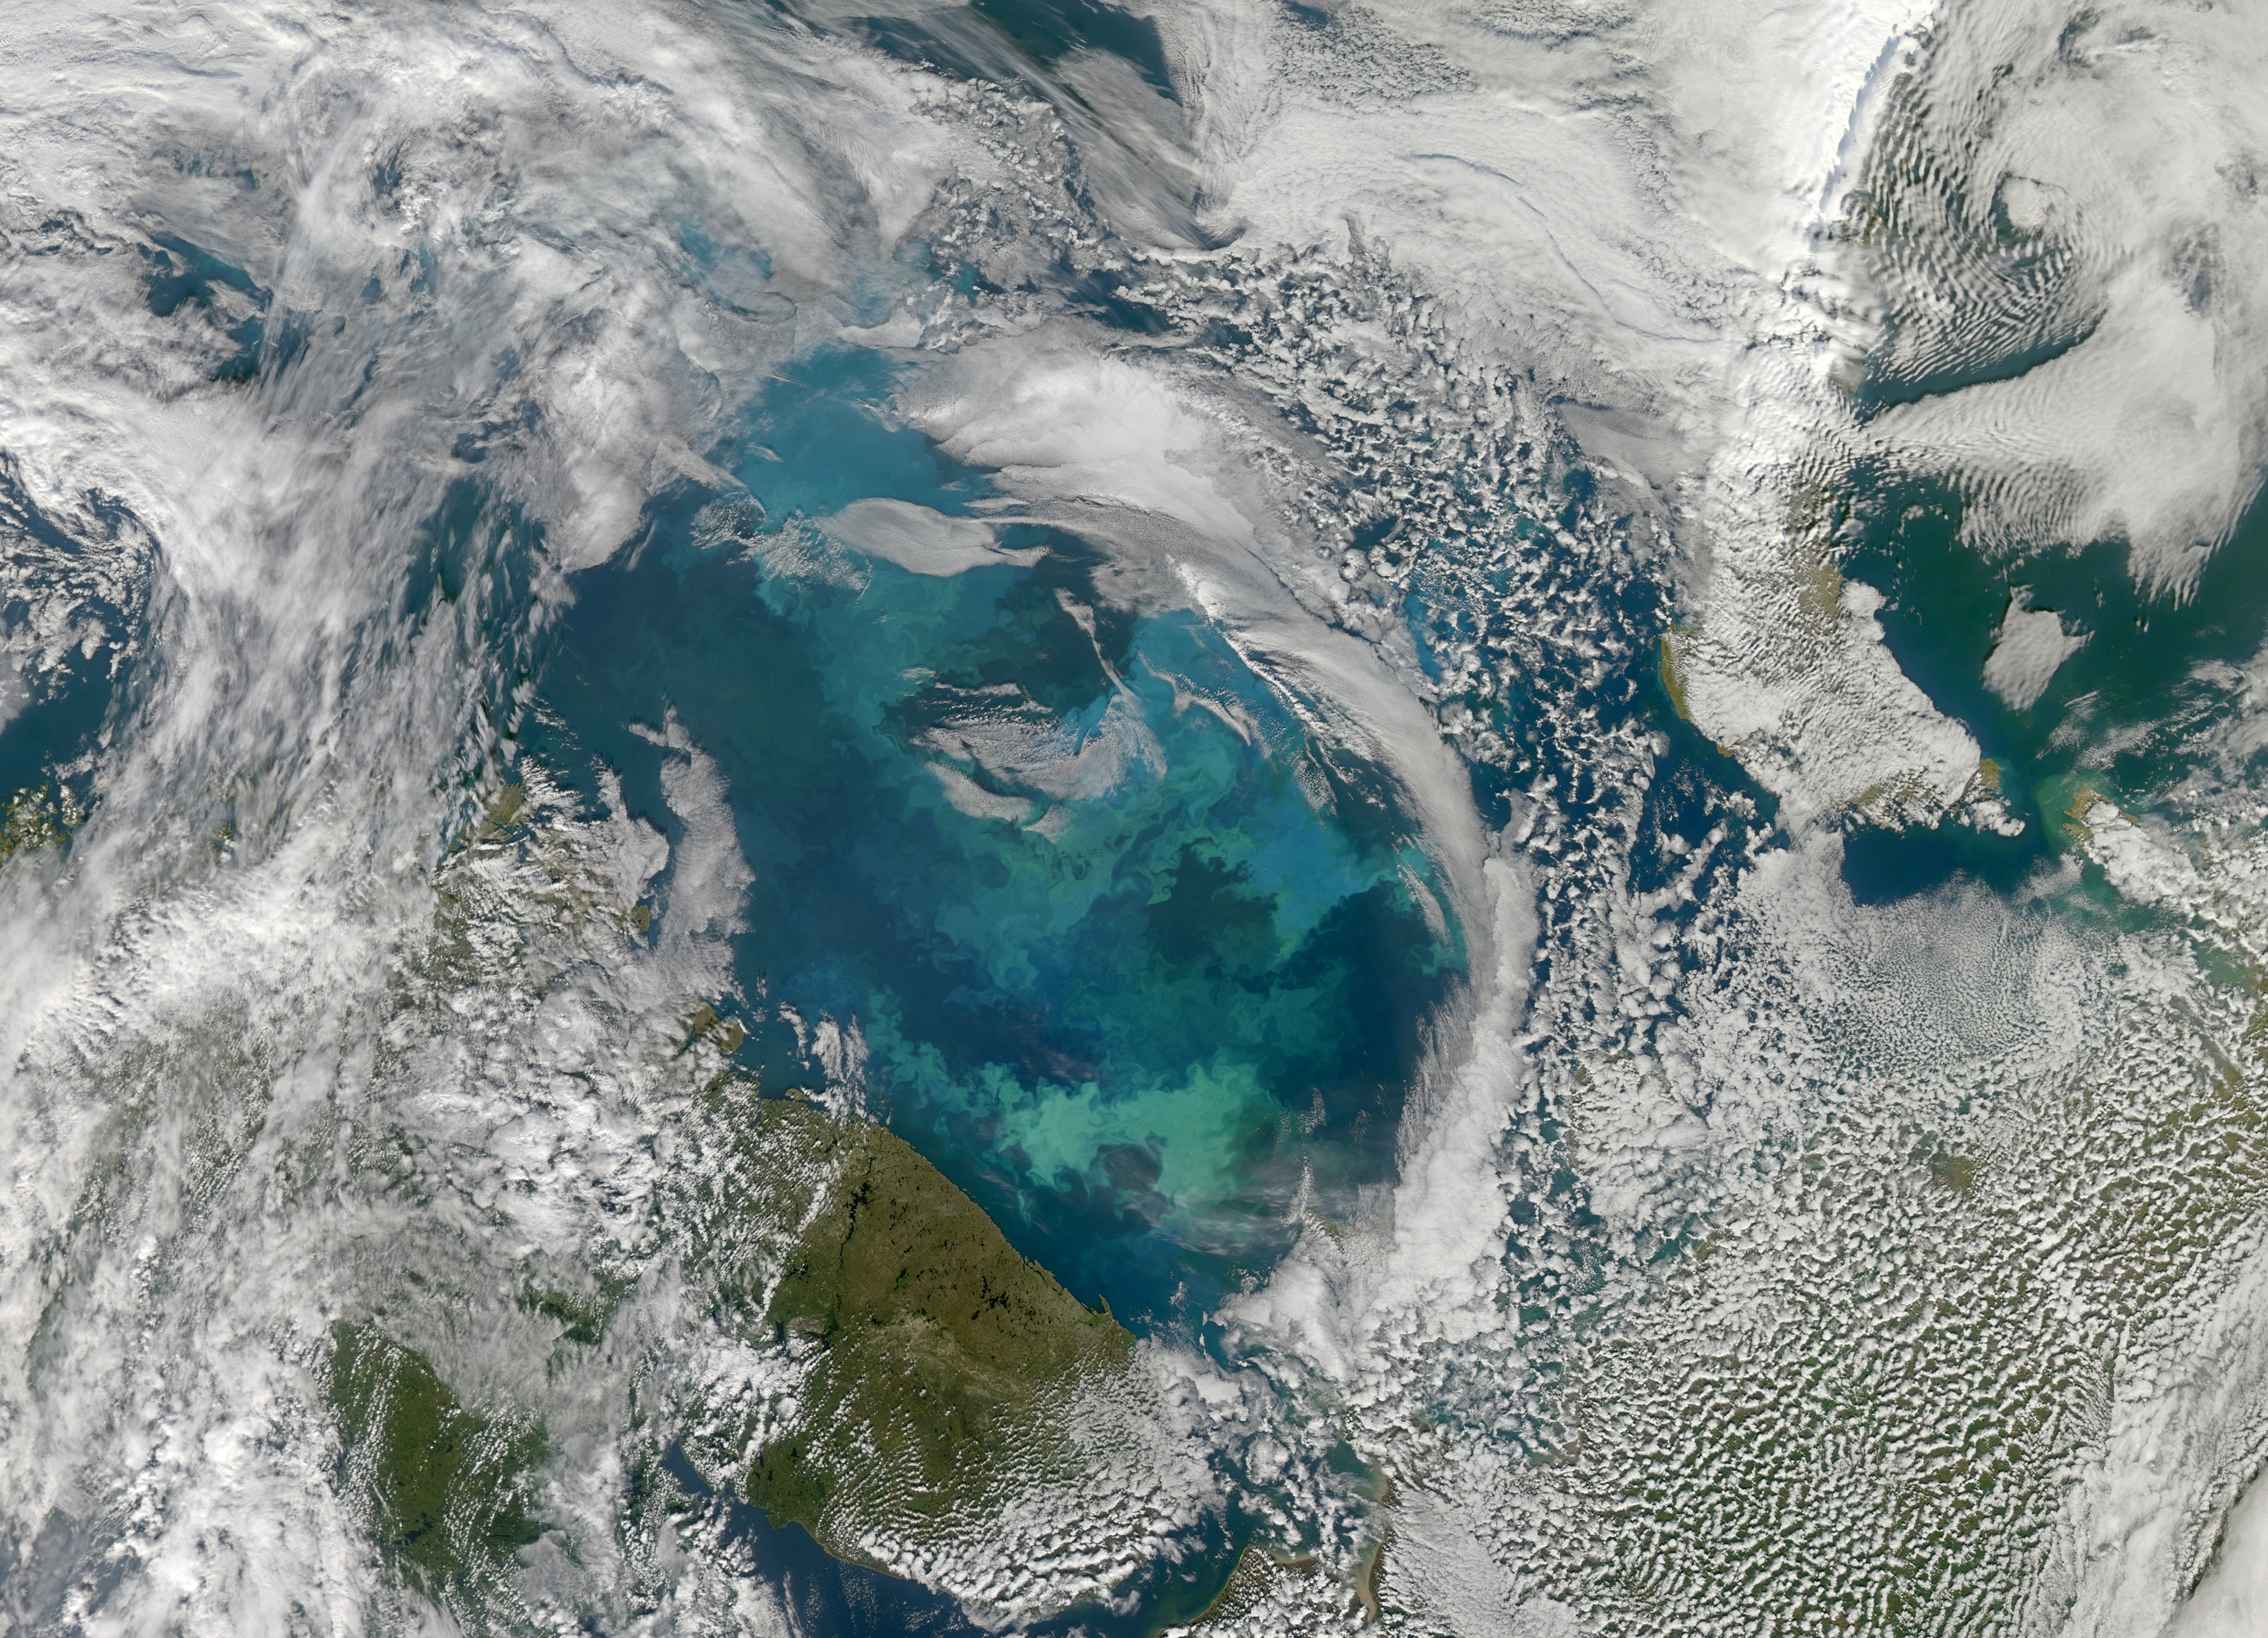
\includegraphics[width=\linewidth]{turb2}}}
\only<3>{\Wider[2em]{\includegraphics[width=\linewidth]{turb3}}}
\only<4>{\Wider[2em]{\includegraphics[width=\linewidth]{turb4}}}
\only<5>{\Wider[2em]{\includegraphics[width=\linewidth]{turb5}}}
\only<6>{\Wider[2em]{\includegraphics[width=\linewidth]{turbm}}}
\end{frame}